In this section, after a brief introduction to COCOMO II, we present
the application of the method to myTaxiService system in order to
get the effort estimation and the expected duration of the project.


\subsection{COCOMOII approach}

Mainly taken from {[}6{]}.

COCOMO II is an updated version of COCOMO 81 which is based on a linear
regression model of the function relating the size of the project
and the effort. However the original version was affected by old time
and non realistic assumptions on the \emph{software lifecycle}, in
particular it assumed that the development process followed the traditional
waterfall scheme, that requirements were supposed to be stable during
the project duration and that the documentation was written incrementally.
COCOMO II is able to overcome those limitation and provide a reasonable
estimation of both the effort and the duration of the project. In
the following subsection we will describe the model.


\subsubsection{Effort Equation}

In COCOMO II \emph{effort} is expressed as \emph{Person-Months} (PM).
\footnote{A person month is the amount of time one person spends working on
the software development project for one month. COCOMO II treats the
number of person-hours per person-month, PH/PM, as an adjustable factor
with a nominal value of 152 hours per Person-Month.%
}The \emph{Effort equation} allows to compute the effort as a function
of the \emph{size} of software development expressed in KSLOC (thousand
of SLOC)%
\footnote{The SLOC in COCOMO represent only the line of codes that are going
to be delivered and they have to be computed as \emph{logical} SLOC.%
} that can be obtained by the Function Points method, a constant, A,
an exponent, E, and a number of values called\emph{ effort multipliers}
(EM). The number of effort multipliers depends on the model. 

\[
Effort=PM=A\cdot Size^{E}\cdot\prod_{i=1}^{n}EM_{i}
\]


where $A=2.94$ for COCOMO II. We now present how to compute $E$
and each $EM_{i}$%
\footnote{Sometimes the overall contribution of the $EM_{i}$ is called $EAF$
(Effort Adjustment Factor) which is trivially defined as $EAF=\prod_{i=i}^{n}EM_{i}$.%
}.


\subsubsection{Software Scale Drivers}

The exponent E in the effort equation is an aggregation of five \emph{scale
factors} (SF, also referred to \emph{scale drivers} SD) is related
to economic, organizational and technical aspects of the environment
in which the project is going to be developed. In particular if account
for the relative economies or diseconomies of scale encountered for
software projects of different sizes {[}Banker et al. 1994{]}. %
\footnote{If E$<$1.0, the project exhibits economies of scale. If the product’s
size is doubled, the project effort is less than doubled. The project’s
productivity increases as the product size is increased. Some project
economies of scale can be achieved via project-specific tools (e.g.,
simulations, testbeds). For small projects, fixed start-up costs such
as tool tailoring and setup of standards and administrative reports
are often a source of economies of scale. If E$=$1.0, the economies
and diseconomies of scale are in balance. This linear model is often
used for cost estimation of small projects. If E$>$1.0, the project
exhibits diseconomies of scale.%
}

The value of E is a contribution of the following scale factors.
\begin{lyxlist}{00.00.0000}
\item [{PREC}] \emph{Precedentedness}: reflects the previous experience
of the organization with this type of project. Very low means no previous
experience, Extra high means that the organization is completely familiar
with this application domain.
\item [{FLEX}] \emph{Development Flexibility}: reflects the degree of flexibility
in the development process. Very low means a prescribed process is
used; Extra high means that the client only sets general goals.
\item [{RESL}] \emph{Architecture / Risk Resolution}: reflects the extent
of risk analysis carried out. Very low means little analysis, Extra
high means a complete a thorough risk analysis.
\item [{TEAM}] \emph{Team Cohesion}: reflects how well the development
team know each other and work together. Very low means very difficult
interactions, Extra high means an integrated and effective team with
no communication problems.
\item [{PMAT}] \emph{Process Maturity}: reflects the process maturity of
the organization. The computation of this value depends on the CMM
(Capability Maturity Model)%
\footnote{CMM is a development model created to represent the ``maturity''
of software development process as the degree of formality and optimization
of processes, from ad hoc practices, to formally defined steps, to
managed result metrics, to active optimization of the processes. Nowadays
the extension CMMI (Capability Maturity Model Integration) is used.%
} Questionnaire but an estimate can be achieved by subtracting the
CMM process maturity level from 5. 
\end{lyxlist}
The following table provides the rating levels for the COCOMO II scale
factors. The selection of scale factors is based on the rationale
that they are a significant source of exponential variation on a project’s
effort or productivity variation. Each scale factors has a range of
rating levels, from Very Low to Extra High and each rating level has
a weight.

\medskip{}


\noindent \begin{center}
\begin{tabular}{c|>{\centering}p{1.5cm}|>{\centering}p{1.5cm}|>{\centering}p{1.5cm}|>{\centering}p{1.5cm}|>{\centering}p{1.5cm}|>{\centering}p{1.5cm}}
\hline 
\emph{Scale Factor } & \emph{Very Low} & \emph{Low} & \emph{Nominal} & \emph{High} & \emph{Very High} & \emph{Extra High}\tabularnewline
\hline 
\hline 
PREC  & {\small{}thoroughly unprecedented}{\small \par}

\textbf{\small{}6.20} & {\small{}largely unprecedented}{\small \par}

\textbf{\small{}4.96} & {\small{}somewhat unprecedented}{\small \par}

\textbf{\small{}3.72} & {\small{}generally familiar}{\small \par}

\textbf{\small{}2.48} & {\small{}largely familiar}{\small \par}

\textbf{\small{}1.24} & {\small{}thoroughly familiar}{\small \par}

\textbf{\small{}0.00}\tabularnewline
\hline 
FLEX  & {\small{}rigorous}{\small \par}

\textbf{\small{}5.07} & {\small{}occasional relaxation}{\small \par}

\textbf{\small{}4.05} & {\small{}some relaxation}{\small \par}

\textbf{\small{}3.04} & {\small{}general conformity }{\small \par}

\textbf{\small{}2.03} & {\small{}some conformity }{\small \par}

\textbf{\small{}1.01} & {\small{}general goals}{\small \par}

\textbf{\small{}0.00}\tabularnewline
\hline 
RESL & {\small{}little (20\%)}{\small \par}

\textbf{\small{}7.07} & {\small{}some (40\%) }{\small \par}

\textbf{\small{}5.65} & {\small{}often (60\%) }{\small \par}

\textbf{\small{}4.24} & {\small{}generally (75\%) }{\small \par}

\textbf{\small{}2.83} & {\small{}mostly (90\%) }{\small \par}

\textbf{\small{}1.41} & {\small{}full (100\%)}{\small \par}

\textbf{\small{}0.00}\tabularnewline
\hline 
TEAM  & {\small{}very difficult interactions }{\small \par}

\textbf{\small{}5.48} & {\small{}some difficult interactions }{\small \par}

\textbf{\small{}4.38} & {\small{}basically cooperative }{\small \par}

\textbf{\small{}3.29} & {\small{}interactions largely cooperative }{\small \par}

\textbf{\small{}2.19} & {\small{}highly cooperative }{\small \par}

\textbf{\small{}1.10} & {\small{}seamless interactions }{\small \par}

\textbf{\small{}0.00}\tabularnewline
\hline 
PMAT  & {\small{}SW-CMM Level 1 Lower}{\small \par}

\textbf{\small{}7.80} & {\small{}SW-CMM Level 1 Upper }{\small \par}

\textbf{\small{}6.24} & {\small{}SW-CMM Level 2 }{\small \par}

\textbf{\small{}4.68} & {\small{}SW-CMM Level 3 }{\small \par}

\textbf{\small{}3.12} & {\small{}SW-CMM Level 4 }{\small \par}

\textbf{\small{}1.56} & {\small{}SW-CMM Level 5 }{\small \par}

\textbf{\small{}0.00}\tabularnewline
\hline 
\end{tabular}
\par\end{center}

\medskip{}


To have a complete description of the meaning of each scale factor,
please refer to {[}6{]} where also assessment methods are proposed. 

Once the value of each scale factor $SF_{j}$ is determined the value
of the exponent $E$ can be computed using the following formula.

\[
E=B+0.01\cdot\sum_{j=i}^{5}SF_{j}
\]


where $B=0.91$ for COCOMO II. Notice that if all scale factors are
judged as Nominal the resulting exponent value is $E=1.0997$.


\subsubsection{Software Cost Drivers}

\emph{Cost drivers} are used to capture characteristics of the software
development that affect the effort to complete the project. All COCOMO
II cost drivers have qualitative rating levels that express the impact
of the driver on development effort. These ratings can range from
Extra Low to Extra High. Each rating level of every multiplicative
cost driver has a value, called an \emph{effort multiplier} (EM),
associated with it. The EM value assigned to a multiplicative cost
driver's nominal rating is 1.00. All those are intended to be evaluated
in post-architecture/early-design phase and they are organized in
categories, for the complete description refer to {[}6{]}.
\begin{itemize}
\item \emph{Product} factors account for variation in the effort required
to develop software caused by characteristics of the product under
development. A product that is complex, has high reliability requirements,
or works with a large testing database will require more effort to
complete.

\begin{lyxlist}{00.00.0000}
\item [{RELY}] Required Software Reliability 
\item [{DATA}] Data Base Size 
\item [{CPLEX}] Product Complexity 
\item [{RUSE}] Developed for Reusability 
\item [{DOCU}] Documentation Match to Lifecycle Needs
\end{lyxlist}
\item \emph{Personnel} factors have the strongest influence in determining
the amount of effort required to develop a software product. The Personnel
Factors are for rating the development team’s capability and experience
– not the individual. These ratings are most likely to change during
the course of a project reflecting the gaining of experience or the
rotation of people onto and off the project. 

\begin{lyxlist}{00.00.0000}
\item [{ACAP}] Analyst Capability 
\item [{PCAP}] Programmer Capability 
\item [{PCON}] Personnel Continuity 
\item [{AEXP}] Application Experience 
\item [{PEXP}] Platform Experience 
\item [{LTEX}] Language and Toolset Experience 
\end{lyxlist}
\item \emph{Platform} factors refers to the target-machine complex of hardware
and infrastructure software (previously called the virtual machine).
The factors have been revised to reflect this as described in this
section. Some additional platform factors were considered, such as
distribution, parallelism, embeddedness, and real-time operations. 

\begin{lyxlist}{00.00.0000}
\item [{TIME}] Time Constraint 
\item [{STOR}] Storage constraint
\item [{PVOL}] Platform Volatility 
\end{lyxlist}
\item \emph{Project} factors account for influences on the estimated effort
such as use of modern software tools, location of the development
team, and compression of the project schedule. 

\begin{lyxlist}{00.00.0000}
\item [{TOOL}] Use of Software Tools 
\item [{SITE}] Multisite Development 
\item [{SCED}] Required Development Schedule 
\end{lyxlist}
\end{itemize}

\subsubsection{Schedule estimation }

The \emph{Schedule equation} allows to determine the \emph{Time to
Develop}, TDEV, expressed in number of months required to complete
the software project.

\[
Duration=TDEV=C\cdot(PM)^{(D+0.2(E-B))}
\]


where $C=3.67$, $D=0.28$, $B=0.91$.

C is a TDEV coefficient that can be calibrated, $PM$ is the estimated
effort, D is a TDEV scaling base exponent that can also be calibrated.
E is the effort scaling exponent derived as the sum of project scale
factors and B as the calibrated scale factor base-exponent. If we
also know the average monthly salary $S$ of the personnel we can
estimate the personnel cost.%
\footnote{Notice that this is very different from the overall cost of the project
since we do not take into account overheads (buildings, heating, lighting,
...).%
}

\[
Cost=PM\cdot S
\]



\subsubsection{Number of people estimation }

Using PM and TDEV calculated before we can give an estimation of the
number of required people.

\[
N=\frac{PM}{TDEV}
\]



\subsection{COCOMO II calculation}

In this subsection we perform the COCOMO II estimation starting from
the SLOC determined in the previous stage thanks to Function Points
approach. Given the academic context and the fact that implementation
was not performed we will try to both perform the calculation with
\begin{itemize}
\item all SFs and CDs rated as nominal and
\item SFs and CDs rated according our opinion with respect to a reasonable
implementation phase.
\end{itemize}
Then we compere the results obtained by the two different approaches.
We also assume that each person involved in the project is payed 2500\$
per month. To easily compute the PM and TDEV we refer to the online
tool \url{http://csse.usc.edu/tools/COCOMOII.php}.


\subsubsection{COCOMO II with all SFs and CDs nominal}

If we assume to set all SFs and CDs to nominal we get the parameters
$E=1.0997$ and $EAF=1$ therefore knowing that $Size=KSLOC=6.716$
we get the following results.

\[
Effort=PM=2.94\cdot(6.716)^{1.0997}\cdot1=23.9\;\mathrm{person-month}
\]


\[
Duration=TDEV=3.67\cdot(23.9)^{0.31794}=10.5\;\mathrm{months}
\]


\[
Cost=23.9\cdot2500\$=59684\;\mathrm{\$}
\]


\[
N=\frac{23.9}{10.5}=2.276\;\mathrm{person}
\]


We report some tables and graphs taken from the web site.

\textbf{Acquisition Phase Distribution}

\noindent \begin{center}
\begin{tabular}{>{\centering}p{2.5cm}||>{\centering}p{2.5cm}|>{\centering}p{2.5cm}|>{\centering}p{2.5cm}|>{\centering}p{2.5cm}}
\hline 
\textbf{Phase} & \emph{Effort (Person-months) } & \emph{Schedule (Months)} & \emph{Average Staff } & \emph{Cost (Dollars)}\tabularnewline
\hline 
\hline 
\textcolor{red}{Inception} & 1.4 & 1.3 & 1.1 & 3581\tabularnewline
\hline 
\textcolor{magenta}{Elaboration} & 5.7 & 3.9 & 1.5 & 14324\tabularnewline
\hline 
\textcolor{blue}{Construction} & 18.1 & 6.5 & 2.8 & 45360\tabularnewline
\hline 
\textcolor{green}{Transition} & 2.9 & 1.3 & 2.2 & 7162\tabularnewline
\hline 
\end{tabular}
\par\end{center}

\textbf{Software Effort Distribution for RUP/MBASE (Person-Months)}

\noindent \begin{center}
\begin{tabular}{c||>{\centering}p{2cm}|>{\centering}p{2cm}|>{\centering}p{2cm}|>{\centering}p{2cm}}
\hline 
\textbf{Phase/Activity} & Inception  & Elaboration  & Construction  & Transition\tabularnewline
\hline 
\hline 
\emph{Management} & 0.2 & 0.7 & 1.8 & 0.4\tabularnewline
\hline 
\emph{Environment/CM} & 0.1 & 0.5 & 0.9 & 0.1\tabularnewline
\hline 
\emph{Requirements} & 0.5 & 1.0 & 1.5 & 0.1\tabularnewline
\hline 
\emph{Design} & 0.3 & 2.1 & 2.9 & 0.1\tabularnewline
\hline 
\emph{Implementation} & 0.1 & 0.7 & 6.2 & 0.5\tabularnewline
\hline 
\emph{Assessment} & 0.1 & 0.6 & 4.4 & 0.7\tabularnewline
\hline 
\emph{Deployment} & 0.0 & 0.2 & 0.5 & 0.6\tabularnewline
\hline 
\end{tabular}
\par\end{center}

\textbf{Staffing profile}

\noindent \begin{center}
\begin{figure}[H]
\noindent \begin{centering}
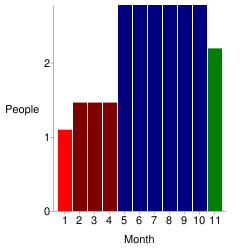
\includegraphics{COCOMOII/images/allnominal}
\par\end{centering}

\protect\caption{COCOMO II histogram - all nominal}
\end{figure}

\par\end{center}

From now on we will discuss how to rate Scale Drivers and Cost Drivers
for myTaxiService.


\subsubsection{Software Scale Drivers}

In the following table we describe for each scale driver the motivations
behind the rating level choice, we refer to the descriptors stated
in {[}6{]}.

\noindent \begin{center}
\begin{tabular}{c|>{\raggedright}p{8.5cm}|>{\centering}p{1.5cm}|>{\centering}p{1.5cm}}
\hline 
\emph{Scale Factor} & \emph{Motivation} & \emph{Rating level} & \emph{Weight}\tabularnewline
\hline 
\hline 
PREC  & \begin{itemize}
\item {\small{}Organizational understanding of product objectives: Thorough}{\small \par}
\item {\small{}Experience in working with related software systems: Moderate}{\small \par}
\item {\small{}Concurrent development of associated new hardware and operational
procedures: Moderate}{\small \par}
\item {\small{}Need for innovative data processing architectures, algorithms:
Some}\end{itemize}
 & Nominal & 3.72\tabularnewline
\hline 
FLEX  & \begin{itemize}
\item {\small{}Need for software conformance with preestablished requirements:
Basic (many aspects were not clearly specified)}{\small \par}
\item {\small{}Need for software conformance with external interface specifications:
Considerable (integration with some external systems needed)}{\small \par}
\item {\small{}Combination of inflexibilities above with premium on early
completion: High}\end{itemize}
 & High & 2.03\tabularnewline
\hline 
RESL & \begin{itemize}
\item {\small{}Percent of development schedule devoted to establishing architecture,
given general product objectives: 25}{\small \par}
\item {\small{}Percent of required top software architects available to
project: 80}{\small \par}
\item {\small{}Tool support available for resolving risk items, developing
and verifying architectural specs: Some}{\small \par}
\item {\small{}Level of uncertainty in key architecture drivers: mission,
user interface, COTS, hardware, technology, performance: Considerable}{\small \par}
\item {\small{}Number and criticality of risk items: Some}\end{itemize}
 & High & 2.83\tabularnewline
\hline 
\end{tabular}
\par\end{center}

\noindent \begin{center}
\begin{tabular}{c|>{\raggedright}p{8.5cm}|>{\centering}p{1.5cm}|>{\centering}p{1.5cm}}
\hline 
\emph{Scale Factor} & \emph{Motivation} & \emph{Rating level} & \emph{Weight}\tabularnewline
\hline 
\hline 
TEAM  & \begin{itemize}
\item {\small{}Consistency of stakeholder objectives and cultures: Strong}{\small \par}
\item {\small{}Ability, willingness of stakeholders to accommodate other
stakeholders’ objectives: Considerable}{\small \par}
\item {\small{}Experience of stakeholders in operating as a team: Considerable}{\small \par}
\item {\small{}Stakeholder teambuilding to achieve shared vision and commitments:
Considerable}\end{itemize}
 & Very High & 1.10\tabularnewline
\hline 
PMAT  & {\small{}Answering to the KPAs (Key Process Area) we get a value of
$KPA%=\ensuremath{30}
$ thus the corresponding EPML (Equivalent Processing Maturity Level)
is 1.5} & Nominal & 4.68\tabularnewline
\hline 
\end{tabular}
\par\end{center}

We obtain a total value for the exponent E of 

\[
E=B+0.01\cdot\sum_{j=i}^{5}SF_{j}=1.0536
\]


Notice that the value of the exponent is smaller with respect to the
one obtained setting all SFs to nominal, this means that we are benefiting
of the quality of the environment in which the software is developed.

\newpage{}


\subsubsection{Software Cost Drivers}

In the following table we describe for each cost driver the motivations
behind the rating level choice, we refer to the descriptors stated
in {[}6{]}. Whenever the information for selecting the most appropriate
rating level is not available we adopt nominal value.

\noindent \begin{center}
\begin{tabular}{c|>{\raggedright}p{8cm}|>{\centering}p{1.5cm}|>{\centering}p{1.5cm}}
\hline 
\emph{Cost Driver } & \emph{Motivation} & \emph{Rating level} & \emph{Effort multiplier}\tabularnewline
\hline 
\hline 
RELY & {\small{}Moderate, easily recoverable losses.} & Nominal & 1.00\tabularnewline
\hline 
DATA & {\small{}10 $\leq$Testing DB bytes/Pgm SLOC$<$100} & Nominal & 1.00\tabularnewline
\hline 
CPLEX & \begin{itemize}
\item \emph{\small{}Control Operations}{\small{}: Highly nested structured
programming operators with many compound predicates. Queue and stack
control. Homogeneous, distributed processing. Single processor soft
real-time control. }{\small \par}
\item \emph{\small{}Computational Operations:}{\small{} Use of standard
math and statistical routines. Basic matrix/vector operations. }{\small \par}
\item \emph{\small{}Device dependent Operations}{\small{}: Operations at
physical I/O level (physical storage address translations; seeks,
reads, etc.). Optimized I/O overlap. }{\small \par}
\item \emph{\small{}Data Management Operations}{\small{}: Multi-file input
and single file output. Simple structural changes, simple edits. Complex
COTS-DB queries, updates. }{\small \par}
\item \emph{\small{}User Interface Management Operations}{\small{}: Simple
use of widget set. }\end{itemize}
 & High & 1.17\tabularnewline
\hline 
RUSE & {\small{}Across program}%
\footnote{“Across project” could apply to reuse across the modules in a single
financial applications project. “Across program” could apply to reuse
across multiple financial applications projects for a single organization.
“Across product line” could apply if the reuse is extended across
multiple organizations. “Across multiple product lines” could apply
to reuse across financial, sales, and marketing product lines.%
} & High & 1.07\tabularnewline
\hline 
DOCU & {\small{}Right-sized to life-cycle needs } & Nominal & 1.00\tabularnewline
\hline 
ACAP & {\small{}Analysts in the 75th percentile} & High & 0.85\tabularnewline
\hline 
PCAP & {\small{}Programmes in the 75th percentile} & High & 0.88\tabularnewline
\hline 
PCON & {\small{}Personell turnover 3\% / year } & Very High & 0.81\tabularnewline
\hline 
AEXP & {\small{}≤ 2 months } & Very Low & 1.22\tabularnewline
\hline 
PEXP & {\small{}≤ 2 months } & Very Low & 1.19\tabularnewline
\hline 
LTEX & {\small{}1 year} & Nominal & 1.00\tabularnewline
\hline 
TIME & {\small{}85\% use of available execution time} & Very High & 1.29\tabularnewline
\hline 
STOR & {\small{}≤ 50\% use of available storage} & Nominal & 1.00\tabularnewline
\hline 
PVOL & {\small{}Major change every 12 mo.; Minor change every 1 mo. } & Low & 0.87\tabularnewline
\hline 
TOOL & {\small{}basic lifecycle tools, moderately integrated } & Nominal & 1.00\tabularnewline
\hline 
SITE & \begin{itemize}
\item \emph{\small{}Collocation Descriptors}{\small{}: Same city or metro.
area }{\small \par}
\item \emph{\small{}Communications Descriptors}{\small{}: Wideband electronic
communication. }\end{itemize}
 & High & 0.93\tabularnewline
\hline 
SCED & {\small{}Shedule compression 130\% of nominal } & High & 1.00\tabularnewline
\hline 
\end{tabular}
\par\end{center}

We obtain a total value for the EAF of

\[
EAF=\prod_{i=i}^{n}EM_{i}=1.149
\]


Note that the value of EAF is grater than the one obtained assuming
all CDs as nominal, this mean that CDs turn out to affect negatively
the overall effort.


\subsubsection{Effort estimation and schedule estimation}

Considering the values computed above, $E=1.0536$ and $EAF=1.149$,
and knowing that $Size=KSLOC=6.716$ we get the following results.

\[
Effort=PM=2.94\cdot(6.716)^{1.0536}\cdot1.149=25.1\;\mathrm{person-month}
\]


\[
Duration=TDEV=3.67\cdot(25.1)^{0.30872}=13.8\;\mathrm{months}
\]


\[
Cost=25.1\cdot2500\$=62832\;\mathrm{\$}
\]


\[
N=\frac{25.1}{13.8}=1.82\;\mathrm{person}
\]


Note that this second result is just slightly different with respect
to the one obtained with all nominal SFs and CDs, in fact the effort
here is grater of 1.2 person-month and also the duration is increased
of 3.3 months; however the required number of people is still around
2. 

We report some tables and graphs taken from the web site.

\textbf{Acquisition Phase Distribution}

\noindent \begin{center}
\begin{tabular}{>{\centering}p{2.5cm}||>{\centering}p{2.5cm}|>{\centering}p{2.5cm}|>{\centering}p{2.5cm}|>{\centering}p{2.5cm}}
\hline 
\textbf{Phase} & \emph{Effort (Person-months) } & \emph{Schedule (Months)} & \emph{Average Staff } & \emph{Cost (Dollars)}\tabularnewline
\hline 
\hline 
\textcolor{red}{Inception} & 1.5 & 1.7 & 0.9 & 3770\tabularnewline
\hline 
\textcolor{magenta}{Elaboration} & 6.0 & 52. & 1.2 & 15080\tabularnewline
\hline 
\textcolor{blue}{Construction} & 19.1 & 8.6 & 2.2 & 47753\tabularnewline
\hline 
\textcolor{green}{Transition} & 3.0 & 1.7 & 1.7 & 7540\tabularnewline
\hline 
\end{tabular}
\par\end{center}

\textbf{Software Effort Distribution for RUP/MBASE (Person-Months)}

\noindent \begin{center}
\begin{tabular}{c||>{\centering}p{2cm}|>{\centering}p{2cm}|>{\centering}p{2cm}|>{\centering}p{2cm}}
\hline 
\textbf{Phase/Activity} & Inception  & Elaboration  & Construction  & Transition\tabularnewline
\hline 
\hline 
\emph{Management} & 0.2 & 0.7 & 1.9 & 0.4\tabularnewline
\hline 
\emph{Environment/CM} & 0.2 & 0.5 & 1.0 & 0.2\tabularnewline
\hline 
\emph{Requirements} & 0.6 & 1.1 & 1.5 & 0.1\tabularnewline
\hline 
\emph{Design} & 0.3 & 2.2 & 3.1 & 0.1\tabularnewline
\hline 
\emph{Implementation} & 0.1 & 0.8 & 6.5 & 0.6\tabularnewline
\hline 
\emph{Assessment} & 0.1 & 0.6 & 4.6 & 0.7\tabularnewline
\hline 
\emph{Deployment} & 0.0 & 0.2 & 0.6 & 0.6\tabularnewline
\hline 
\end{tabular}
\par\end{center}

\textbf{Staffing profile}

\noindent \begin{center}
\begin{figure}[H]
\noindent \begin{centering}
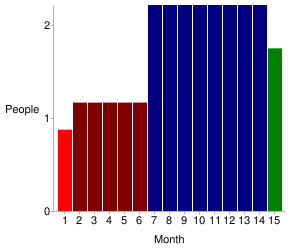
\includegraphics{COCOMOII/images/real}
\par\end{centering}

\protect\caption{COCOMO II histogram}
\end{figure}

\par\end{center}
